\chapter{Implementation}

\label{chap:impl}

% -------------------------------------------------------------------------------------------------
%                                           General TODOs
% -------------------------------------------------------------------------------------------------


\todo{Add references to documentation at appropiate places}
\todo{ add disclaimer, that most of this information was derived from reading the source code and may in some places not be accurate because the code is pretty complex and
    i have only been at it for a few months}

% TODO viruteller address raum eines xv6 processes
% Qemu implementation TLB vs Echter TLB
% -------------------------------------------------------------------------------------------------
%                                    Chapter structure overview
% -------------------------------------------------------------------------------------------------

%   Source overview
%     QEMU
%     xv6
%   Stage1 - Single Fixed address
%     Qemu - exception
%     xv6 - tlb triggerer
%   Stage2
%     Qemu - TLB CSRs
%     xv6 - Exception Handler, single address tlb fill
%   Stage3 - VM PTW with TLB miss handler
%     Qemu -> Extension to all addresses
%     xv6 -> tlb miss handler with ptw
%       Exception vector entry -> state save, kernel stack
%   Stage4 - Dynamic Segmentation allocation scheme (btw -> link to MIPS?)
%     Qemu -> No more changes needed
%     xv6 -> A lot of changes here
%   Debugging
%   Discussion on implementation
%       Concurrency
%       VM Features
% -------------------------------------------------------------------------------------------------

% High level description of the development steps and their reasoning

% -------------------------------------------------------------------------------------------------
% Section on the rationale for choosing this platform -> or just say that this was chosen and dont rationalize it

% -------------------------------------------------------------------------------------------------
% Introductory section
This chapter summarizes the implementation of the softtlb page-table-less virtual memory system.
The ordering of the sections in this chapter reflect the implementation process and will thus
be comprised of following steps:
\begin{enumerate}
    \item \textbf{TLB Miss Exception and Exception Triggerer} The first step is about
          the implementation of the TLB Miss Exception in the QEMU RISC-V emulator. On the xv6-side,
          a user-mode program is added to trigger a TLB Miss exception from the shell.
    \item \textbf{Exception Handling and TLB Writing} The second step implements the
          handling of the TLB Miss Exception, by implementing a machine mode exception handler.
          The RISC-V emulation is extended by two new CSRs that facilitate writing TLB from the
          software-side of things.
    \item \textbf{Software Page Table Walk for all Addresses} This step removes the restriction
          in the QEMU emulator to only throw exeptions for a specific address. In the exception handler,
          a page table walk is implemented to now create virtual to physical mappings for all addresses.
    \item \textbf{Segmented Memory Design using software-defined TLB Filling} In this step, the xv6 virtual memory system is completely
          replaced. The new design gets rid of the page table and only uses information present in
          registers to create virtual-to-physical mappings and to fill the tlb.\\
\end{enumerate}
Each section elaborates on both the xv6 side and the QEMU side of the implementation.\\
The final section describes debugging techniques that were used or can otherwise be useful for
similar implementations.



% First step in the development process
% -------------------------------------------------------------------------------------------------
%                                          SECTION STEP 1
% -------------------------------------------------------------------------------------------------
\section{TLB Miss Exception and Exception Triggerer }
There are two requisites the hardware needs to fulfill in order to do a software-managed TLB fill:
There needs a way to signal the operating system that a TLB miss occured and there needs to be some
sort of instruction that can be used to write TLB entries.\\
This step is about the former: Changing the QEMU RISC-V emulator to throw a newly defined \textit{
    TLB MISS Exception} whenever the TLB misses.\\
% Why only start with one fixed address?
Changing the whole system to start throwing a TLB Miss Exception on every virtual address would
make it very hard to debug both first tries at implementing a handler for the exception and the
exception throwing code in QEMU itself.\\
And not only would the exception be thrown as soon as virtual memory is activated in
\texttt{xv6-riscv:kernel/main.c}, the exception would be thrown
as soon as exceptions are activated and a memory access happens, because QEMU also uses the
\texttt{fill\_tlb} routine to fill the TLB with direct
virtual-to-physical mappings when no virtual memory is used. This speeds up the execution of
the dynamically-translated code, as it can directly
lookup addresses in the TLB using a fast path \cite{DeepDiveQEMU}.\\ \todo{add: dynamically-generated tcg code can
    directly use the TLB structures}\\
For this step of the implementation, the QEMU memory system emulation must be changed to throw a
TLB Miss Exception when a TLB lookup misses. To keep the system running as normal, this will
be done for only one hardcoded address, that is usually not used by xv6.\\
On the xv6 side, we need a user-level program, that accesses the specific address and thus prompts
the emulated hardware to throw a TLB Miss exception.


% -------------------------------------------------------------------------------------------------
\subsection{Address Selection}
The choice for an address to be used for testing the TLB Miss exception throwing is easy:
As shown in Figure \ref{impl:xv6layout} \cite{cox2011xv6}, the physical memory map of xv6 has a
area of ''Free memory'' that is managed by the physical memory allocator. The memory allocator
always gives out the next page starting from low to high addresses when a new page is requested
by kernel routines. The address \texttt{0x84fff000} was chosen as a testing address.\\
Note that the physical memory allocator in \texttt{kalloc.c} will actually touch an this (or
any address in the range from \texttt{0x80000000} to \texttt{0x88000000}), when initializing
the linked list used to keep track of the free pages \cite{cox2011xv6}.\todo{explain why this
    may be relevant or just leave it out? }
% does not need to be a accessible address now, but later we want to write and read from it

\begin{figure*}[t!]
    \centering
    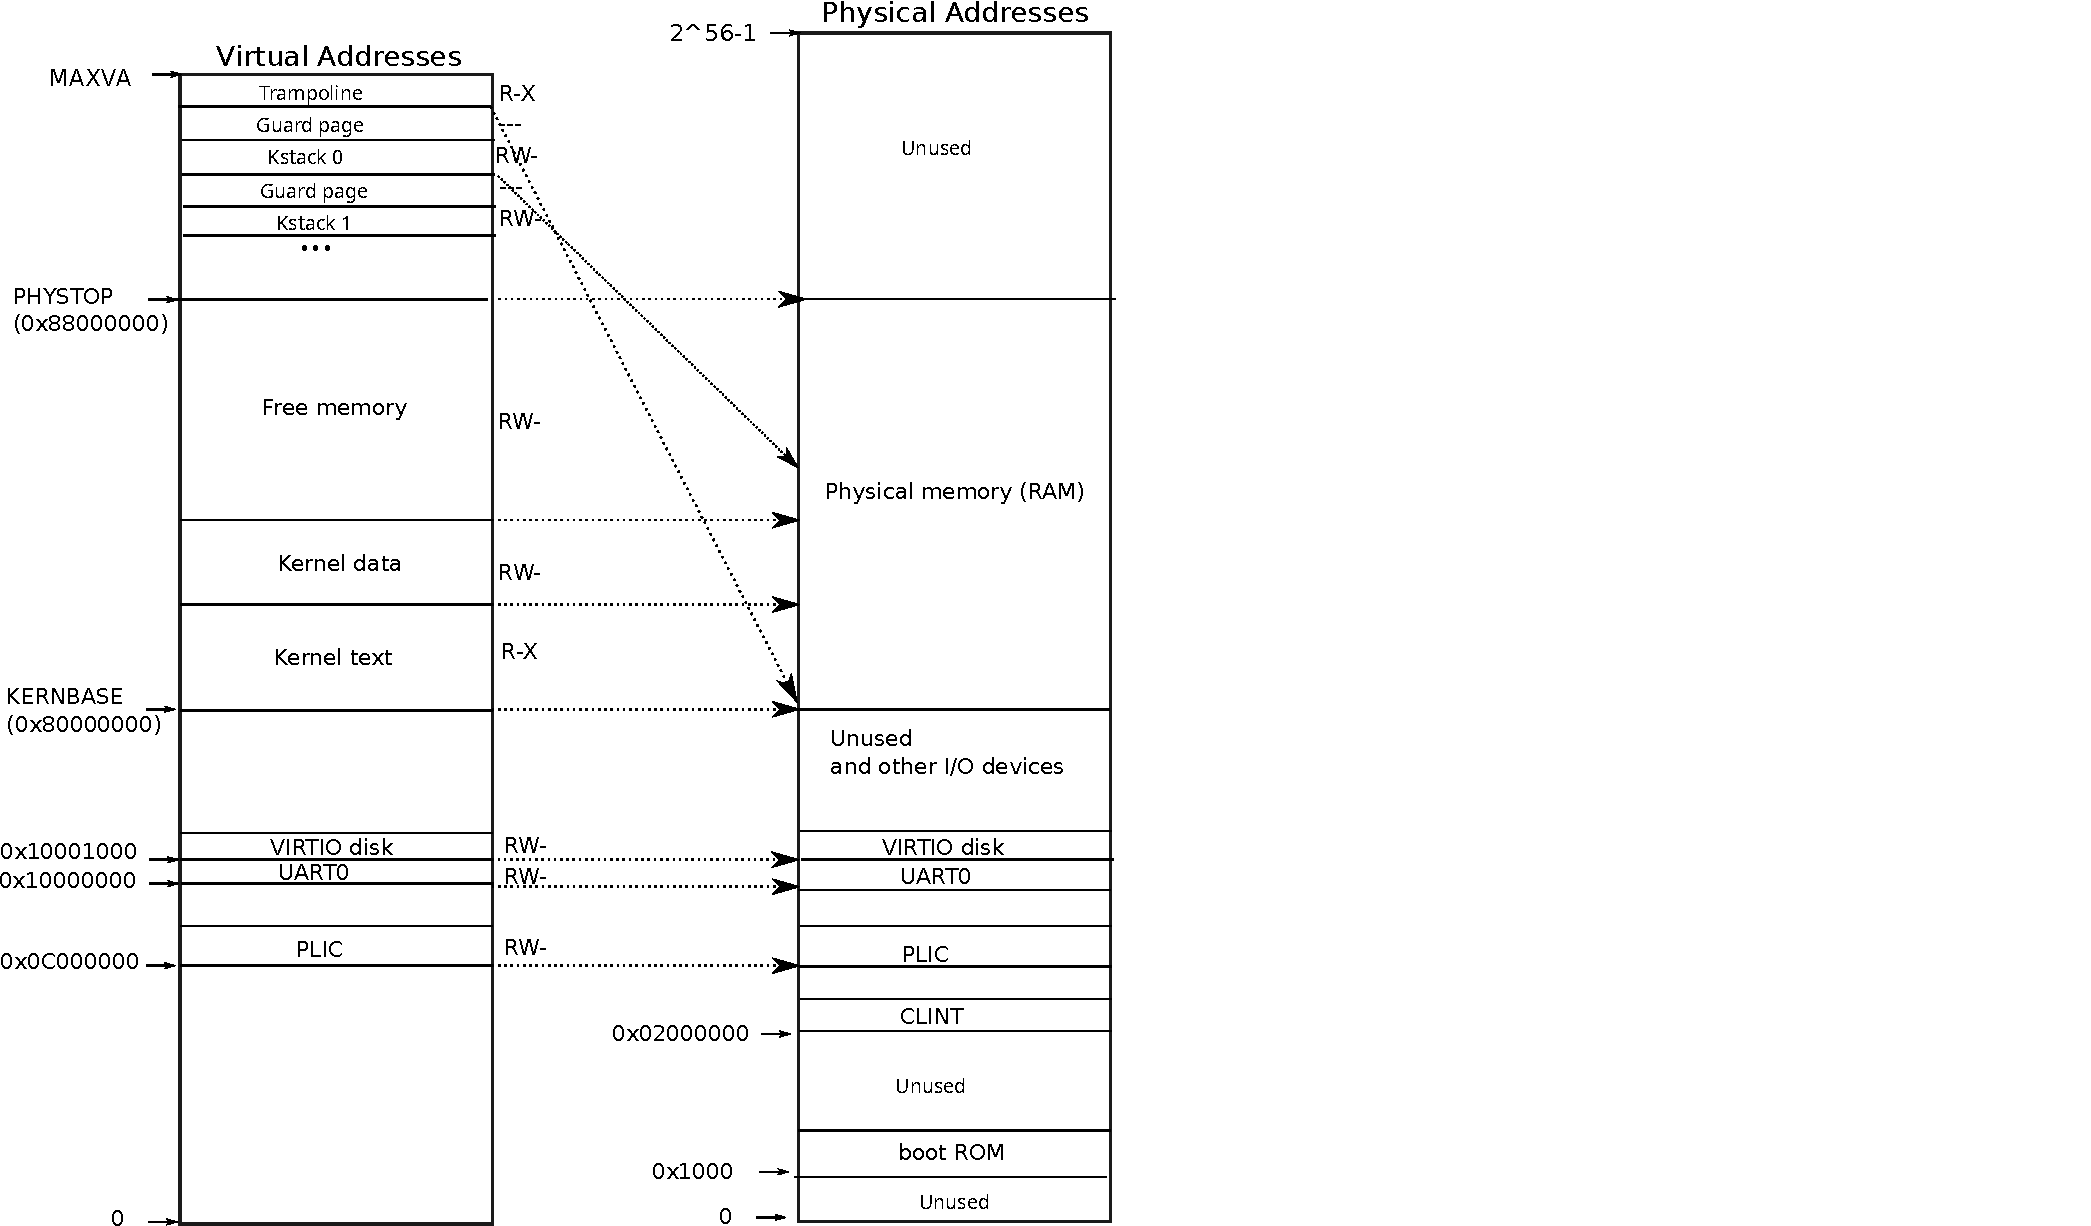
\includegraphics[scale=.5]{figures/xv6_layout.pdf}
    \caption[xv6 memory layout]{The xv6 memory layout and how the kernel virtual address space is mapped on
        the physical address space. Taken from the xv6 book \cite{cox2011xv6}.}
    \label{impl:xv6layout}
\end{figure*}


\subsection{TLB Miss Exception in QEMU}
%TODO Explain what the riscv_cpu_tlb_fill function does originally - in detail
% TODO discussion and reference to READER/SPECIFICATION on what exception numbers and other constants can be used and are free

% Qemu RISCV  exception adding "tutorial"
%TODO Description of the TLB Exception implementation and how to generally add exceptions to the QEMU plattform
% TODO List of code locations where changes need to be added -> should be usable as back reference for implementing more exceptions

To properly test the implementation, the \texttt{tlb\_fill} function was replaced to throw the
TLB\_MISS exception for
one specified, page-aligned address and to continue on normally for every other address.
The implementation is outlined
in Listing \ref{lst:specialCaseTLBfill}.



% riscv_cpu_tlb_switch function 
%TODO is this listing really interesting?
\begin{lstlisting}[language=c,float=h!,
    caption={Alternative Implementation for the RISC-V tlb\_fill function with a special case to
    start testing TLB Miss Handler implementations.\\
    In line 11, a conditional branch is used to only trigger the exception when neither the
    Virtual Memory (as set in the \texttt{satp} \texttt{MODE} field) is bare nor the priviledge
    mode is the machine mode.\\
    If the virtual address is the hardcoded one, a TLB Miss exception is thrown, otherwise the
    original functions is called, which will perform a page table walk to find the mapping.},
    label={lst:specialCaseTLBfill}]
bool my_riscv_cpu_tlb_fill(CPUState *cs, vaddr address, int size,
    MMUAccessType access_type, int mmu_idx,
    bool probe, uintptr_t retaddr)
{
    RISCVCPU *cpu = RISCV_CPU(cs);
    CPURISCVState *env = &cpu->env;
    int mode = mmuidx_priv(mmu_idx);
    int vm = get_field(env->satp, SATP64_MODE);
    bool ret = false;

    if(!(vm == VM_1_10_MBARE || mode == PRV_M) &&
            address == (uint64_t)0x84fff000) {
        ret = riscv_cpu_tlb_miss_exception(cs,address,size,access_type, mmu_idx, probe, retaddr);
    } else {
        ret =  riscv_cpu_tlb_fill(cs,address,size,access_type, mmu_idx, probe, retaddr);
    }
    return ret;
}
\end{lstlisting}

% -------------------------------------------------------------------------------------------------


% This section describes the necesarry steps for adding the tlb miss exception to the qemu source
%in comparison with Page fault exceptions
To draw inspiration on how to implement a TLB Miss exception in QEMU, you can take a look at how
page fault exceptions are thrown.\\
Whenever a page fault exception is triggered, the TLB is checked first to see if there is a mapping
for the input virtual address \cite{QEMUSource2024}. Additionally, RISC-V cores provide the faulting
address of the page fault exception in the \texttt{mtval} register \cite{RISCVInstructionSet}.\\
The faulting address will also be necessary for handling the TLB Miss exception.


% -------------------------------------------------------------------------------------------------

% -------------------------------------------------------------------------------------------------

% Adding new Exception to Qemu RV target
\paragraph{Adding a new exception}to the QEMU emulator requires changes at a number of places. In the following,
the relevant code locations in the QEMU source \cite{QEMUSource2024} are shown.\\
This may be completely different for other targets, as the exception code is mostly target specific and
this implementation only looked at the RISC-V target.
\begin{itemize}
    \item \texttt{target/riscv/cpu\_bits.h} contains all CPU-definitions specific to the RISC-V target.
          There is also a enum called \texttt{RISCVException} which contains the number-codes for all RISC-V exceptions.
          In choosing a appropiate number for a new exception, one should consult the Privileged Architecture Specification \cite{RISCVInstructionSet}.
          There are specific exception code ranges that are designated for custom use. E.g. the codes 24--32 and 48--63.
    \item \texttt{target/riscv/cpu\_helper.c\:riscv\_cpu\_do\_interrupt\(\)} is the target-specific function
          for triggering interrupts. Here it suffices to add the new exception enum item to the switch case, when
          the new exception is similar in behavior to exising exceptions.\\
          Here the new exception is simply supposed to jump into an exception handler in the kernel. A lot of exceptions
          like page faults share that behavior.
    \item Finally, if the exception should be delegatable to supervisor mode or user mode, the n-th bit,
          with n being the exception code, needs to be set in the \texttt{DELEGABLE\_EXCPS} definition in \texttt{target/riscv/csr.c}.
          This enables the kernel to delegate the exception to another priviledge level by setting the appropiate
          bit in the \texttt{medeleg} and \texttt{sedeleg} CSRs.
\end{itemize}

The code shown in Listing \ref{lst:specialCaseTLBfill} will finally trigger the function shown in
Listing \ref{lst:exceptionThrow}.\\ After executing this function, QEMU will trigger a TLB Miss exception as soon
as it gets back to the main execution loop \cite{QEMUSource2024}.

\begin{lstlisting}[language=c,float=h!,
    caption={Setup-Code for raising a TLB Exception. The \texttt{cs-\textgreater exception\_index} variable needs
    to be set to the custom \texttt{TLB Exception} enum value. The \texttt{env-\textgreater badaddr} variable
    will end up in the \texttt{mtval} register. The address will be page-aligned first, by zeroing out the
    lowest 12 bits. This is used to encode the \texttt{mmu\_idx} into the faulting address. Why this is
    necessary is explained in Section \ref{sect:tlbwrite}},
    label={lst:exceptionThrow}]

    static void raise_tlb_exception(CPURISCVState *env, target_ulong address,
                                MMUAccessType access_type,
                                /*unnecessary?*/ bool pmp_violation,
                                bool first_stage, bool two_stage,
                                bool two_stage_indirect, uint8_t mmu_idx) {
        CPUState *cs = env_cpu(env);

        cs->exception_index = RISCV_EXCP_TLB_MISS;
        env->badaddr = ( address & ~( (1 << 12) - 1)) | mmu_idx;
        env->two_stage_lookup = two_stage;
        env->two_stage_indirect_lookup = two_stage_indirect;
    }

\end{lstlisting}

% -------------------------------------------------------------------------------------------------


\subsection{Exception Triggerer}
% TODO TLB exception trigger
To properly test the changes introduced to the QEMU emulator, there needs to be some way to
trigger a TLB exception.\\
By implementing this as a user-level program, the exception can be triggered using the xv6 shell.

\textbf{Adding a new user-level Program to xv6} only needs you to add a new \texttt{.c} file to the user subfolder
and to add the name of the generated binary ( name of \texttt{.c} file prefixed with a \texttt{\_})
to the list of user binaries in the makefile.\\
The new \texttt{.c} file only needs a \texttt{main} function and should also include the \texttt{user.h}
file to gain access to some preimplemented function and system call wrappers \cite{xv6source}.

The final exception triggerer may look something like this:

\begin{lstlisting}[language=c,float=h!,label{impl:excptTrigger},caption={\textbf{Exception Triggerer} Trying to
    load from a hardcoded address prompts the emulated hardware to trigger a TLB Miss Exception.}]
    #include "kernel/types.h"
    #include "user/user.h"

    void do_tlb_exc(void) {
        __asm__("li s2, 0x84fff000\n\t \
                lw s4, 0(s2)\n\t");
        register int *foo asm ("s4");
        printf("%x\n", foo);
        return;
    }
    
    int main(int argc, char *argv[]) {
        do_tlb_exc();
        //exit(0);
    }
\end{lstlisting}
The program first loads the hardcoded address into a register and then tries to load a word from this address.
If the implementation of the \texttt{TLB Miss Exception} was done correctly, the process will trap to the kernel
and the kernel will print out an error message, as it does for all exceptions that either have unknown exception
numbers or do not have a exception handler implemented \cite{cox2011xv6}.\\
If the exception was not properly implemented, the kernel would report a load page fault exception.

\todo{add xv6 shell output at this stage progression - should be a error printed by the kernel exception handler}
% -------------------------------------------------------------------------------------------------
%                                       END OF SECTION - STEP 1
% -------------------------------------------------------------------------------------------------



% Second step: Extending the tlb miss handling to be used for all addresses -> implementing a softvm ptw
% -------------------------------------------------------------------------------------------------
%                                         SECTION - STEP 2
% -------------------------------------------------------------------------------------------------
\section{Exception Handling and TLB Writing}
\label{sect:tlbwrite}

Now that the new \textit{TLB Miss Exception} can be triggered by a user-level program, there needs
to be an exception handler in the kernel that will create virtual-physical mappings and add them to the
TLB.\\
This section will first go into a general description to add new CSRs to the RISC-V QEMU emulation and
will then elaborate on the specific implementation for the TLB CSRs.\\
The section ends with the implementation of the exception handler.

% TODO Why does the mmuidx need to be encoded into the faulting address -> Explain


% -------------------------------------------------------------------------------------------------
\subsection{Adding CSRs to RISC-V/QEMU}

% Relevant Code locations
Following code locations are relevant for CSRs in the RISC-V/QEMU emulation source code \cite{QEMUSource2024}:
\begin{itemize}
    \item \texttt{disas/riscv.c} Contains a big switch case with all the CSR number to CSR name mappings.
          Name and number of new CSRs need to be added there.
    \item \texttt{target/riscv/cpu\_bits.h} contains definitions for all CSR numbers.
          While it is not strictly necessary to add another definition for new CSRs here, readability and maintainability
          of the code increases if a more descriptive definition name is used instead of a magic constant.
    \item \texttt{target/riscv/cpu\_cfg.h} contains a structure called \texttt{RISCVCPUConfig}. Every emulated RISC-V hart
          has this structure to expose all the extensions that the hart supports. \todo{hart already known?}\\
          The structure has a boolean flag for every extension that is currently supported by the emulator.\\
          New extensions should get their own flag in this struct.\\
          Similar entries also need to be added to the \texttt{isa\_edata\_arr} and \texttt{riscv\_cpu\_extensions} arrays in \texttt{target/riscv/cpu.c}.
    \item \texttt{target/riscv/csr.c} contains the implementation for all CSRs. The \texttt{riscv\_csr\_operations csr\_ops[]}
          array is essential for adding callback functions to CSR numbers.\\
          For every new CSR, a struct of the type \texttt{riscv\_csr\_operations} must be added to that array using the
          CSR number as an index. This struct is comprised of multiple function pointers, which deal with
          \begin{itemize}
              \item Checking if the hart implements the CSR
              \item Reading from the CSR
              \item Writing to the CSR
              \item Combined read/write
              \item 128 bit read/writes
          \end{itemize}
\end{itemize}
%Implementation of CSRs

As previously mentioned, the CSRs have some index ranges for new, custom CSRs. For the implementation
of TLB write CSRs, the indexes \texttt{0xBEE} and \texttt{BFF} have been selected.\\
Using these constants and the steps above, two new instructions\todo{are these actually instructions} can be realized.

\subsection{CSR Callback Implementation} Apart from the above mentioned steps to add new CSRs to the emulator, the
main logic of the implementation is in the callbacks referenced in \texttt{target/riscv/csr.c}.\\
The implementation of these callbacks is strongly dependent on the structure of the data that is written to
the CSRs. Fundamentally, these callbacks act as a bridge between the exposed ISA and the implementation of
that instruction set in software.\\
As previously mentioned, two new CSRs will be needed to implement the TLB-writing. \todo{ PUT THIS IN THE THEORY PART about CSR format and number: In theory, it would
    also be possible to implement the functionality using only one CSR, by just taking the faulting address from the mtval register, but
    this paper focuses on the proof of concept of the design and not on the optimization }.\\
The implementations
of the write-callbacks look as follows:


% Callbacks

\begin{lstlisting}[language=c,float=h!,
    label={lst:tlbh}]
    static RISCVException write_tlbh(CPURISCVState *env, int csrno, target_ulong new_val)
    {
        env->tlbh = new_val;
        return RISCV_EXCP_NONE;
    }
\end{lstlisting}
The implementation of the \texttt{tlbh} CSR write, does not do anything else but saving the value
that is written to it to the environment of the CPU.\\
This is because the theory specifies\todo{is it specified yet?}\\, that the TLB entry will only
be written to the TLB when the write to the \texttt{tlbl} CSR has succeeded.

\begin{lstlisting}[language=c,float=h!,
    label={lst:tlbl}]
    static RISCVException write_tlbl(CPURISCVState *env, int csrno, target_ulong pte)
    {
        
        target_ulong tlb_size = TARGET_PAGE_SIZE;
        
        CPUState *cpu = env_cpu(env);
        vaddr addr = env->tlbh;
        hwaddr paddr = ((pte & ~(PTE_RESERVED)) >> 10) << 12;

        int mmu_idx = addr & (tlb_size - 1);

        int prot = pte & (PTE_R | PTE_W | PTE_X | PTE_V );

        addr &= ~(tlb_size - 1);
        paddr &= ~(tlb_size - 1);

        tlb_set_page(cpu, addr, paddr, prot, mmu_idx, tlb_size, false);
        
        env->tlbh = 0;
        env->tlbl = 0;

        return RISCV_EXCP_NONE;
    }
\end{lstlisting}
\todo{all these code lines need a theoretical foundation in the fundamentals chapter (BTW, the format
    still adheres to PTEs!)}
The value written to the \texttt{tlbl} CSR adheres to the same format as the RISC-V Sv39 PTEs (As shown in section \ref{fund:sv39}).

To get the page-aligned physical address and to get rid of the access bits stored in the lower 10 bits,
the value will first be right-shifted by ten and then left shifted by 12 bits.\\
The top most bits are specified to be all zero, as explained in the fundamentals chapter \cite{RISCVInstructionSet}.

In line 10, the \texttt{mmu\_idx} is extracted from the lowest 11 bits of the virtual address. This is
necesarry, because QEMU uses up to 16 different MMU modes with dedicated TLBs \cite{QEMUSource2024}.
Whenever QEMU performs a TLB lookup, it does so in a specific MMU mode. This MMU mode is clear when
a TLB entry is retrieved, it is however not clear when a TLB entry is written.
To still fill the correct TLB, the \texttt{mmu\_idx} is transfered to the exception handler as part
of the faulting address in \texttt{mtval} and then back to the emulator via the TLB write CSRs.

The following lines deal with extracting the protection bits from the PTE and with page-aligning
the virtual and physical addresses. Finally, a preexisting QEMU function is invoked to add
a new entry to the emulated TLB and the CSR values are cleared.\\
The return value \texttt{RISCV\_EXCP\_NONE} indicates that nothing out of the ordinary happend.

This is all that needs to be done to add CSRs for TLB filling to the QEMU RISC-V emulator.


\todo{discussion of implementation at the end of this chapter: shortcommings, comparison QEMU - MIPS, comparison xv6 new vm - other vm -> eval??}

% -------------------------------------------------------------------------------------------------

\subsection{TLB Miss Exception Handler}
% Previous state of xv6 machine mode trap handler
%   -> Only for Timer Interrupt
%   -> Small amount of saved registers
% TODO TLB fill manager
% Changes -> Vectored mode to keep timer interrupt as is, just need to move it
With capabilities to write TLB entries in place, an effective exception handler can be implemented.

\textbf{xv6 Machine-Mode Trap Handler} The xv6 machine-mode trap handler only deals
with the timer interrupt. All other interrupts and exceptions are delegated to the supervisor
mode. This allows the trap handler to be very small and very specific to the timer interrupt \cite{cox2011xv6}.
It thus only needs to store two registers two memory to make enough room in the register file
to reset the timer and invoke the scheduler.\\
Adding another trap to be handled adds more complexity, as the trap number needs to be checked
and the code needs to branch to the right routines.

But it can also be completely avoided to touch the timer code at all. xv6 uses trap vectoring
mechanism in \textit{direct} mode.\\ In direct mode, all traps jump to the same address.
Using the \textit{vectored} mode makes all \textit{exceptions} jump to the address set
in the \texttt{mtvec BASE} field but all \textit{interrupts} are set the program counter
to \texttt{BASE} plus four times the interrupt cause \cite{RISCVInstructionSet}.

So to add machine mode exception handlers with disrupting the existing code as little as possible only
requires changing the trap vectoring mode to \texttt{vectored} mode and moving the timer interrupt code
to the correct offset.

\begin{lstlisting}[language=diff]
-    w_mtvec((uint64)timervec);
+    w_mtvec((uint64)mtvec_vector_table | 0x1);
\end{lstlisting}

The changes for changing the mode are trivial. Only the one bit indicating the \texttt{vectored} mode
needs to be set.\\
Placing the timer vector at the correct offset from the default trap handler vector can be achieved by
filling the space between the base address and the timer vector with no-operations. The same could be
achieved with linker directives.\\
The interrupt number for the timer interrupt is \texttt{0x7}, so thats puts the timer interrupt vector
at a positive \texttt{0x1c} offset from the base address.

\begin{lstlisting}[language={[RISC-V]Assembler},float=h!,
    label={lst:defaultTrapHandler}, caption={Vectored Trap Handler Routine}]
mtvec_vector_table:
IRQ_0:
        j default_exception_handler
        nop
IRQ_1:
        j default_vector_handler
        nop
IRQ_2:
        j default_vector_handler
        nop
IRQ_3:
        j default_vector_handler
        nop
IRQ_4:
        j default_vector_handler
        nop
IRQ_5:
        j default_vector_handler
        nop
IRQ_6:
        j default_vector_handler
        nop
IRQ_7:  # timer handler
        j timervec
\end{lstlisting}

% TODO verifying the placement of addresses and symbols using the name utility

RISC-V provides 4 bytes for every interrupt request (IRQ) and the default trap handler. This is not enough
to implement proper trap handling, so these 4 bytes are typically spent jumping to a more elaborate trap
handling routine.

Now any machine-mode exception (that is not delegated to a lower-priviledge mode) sets the program counter
to the address of the \texttt{mtvec\_vector\_table} label. The next jump brings the execution into
the default exception handler.
The timer interrupt will jump directly to the \texttt{IRQ\_7} label.

\textbf{Store/Load Sandwich} The idea behind the \textit{softtlb} design is to not use as many of the five
memory references modern architectures need for a page table walk \cite{intel5LevelPaging5Level2017}. But
for a first proof of concept, it is helpful to not have to think about which registers to use and to not optimize
away all unnecesarry memory references before the design even works.\\
That is why the first thing the default exception handler will do is to store the current state of the register
file.\\
This is essential so that, once returned to the context that triggered the TLB miss, execution can continue
as if nothing happened.\\
After storing the state and running the exception handler, the state must again be loaded into the registers.

\begin{lstlisting}[language={[RISC-V]Assembler},float=h!,
    label={lst:defaultTrapHandler}, caption={Store/Load Sandwich}]
default_exception_handler:

    csrrw a0, mscratch, a0
    sd sp, 40(a0)

    ld sp, 48(a0)
    csrrw a0, mscratch, a0

    # make room to save registers.
    addi sp, sp, -256

    # save the registers to the hart stack
    sd ra, 0(sp)
    sd gp, 16(sp)
    ...
    sd t5, 232(sp)
    sd t6, 240(sp)

    addi s0, sp, 256 # Set Frame Pointer

    # ??
    # csrr t0, sscratch
    # sd t0, 8(sp)

    # TODO Pass args to fx

    # csrr a0, mtval
    # csrr a1, satp

    call machine_default_exception_handler 


    # restore registers from hart stack
    ld ra, 0(sp)
    ld gp, 16(sp)
    ...
    ld t5, 232(sp)
    ld t6, 240(sp)

    addi sp, sp, 256
    
    csrrw a0, mscratch, a0

    sd sp, 48(a0)
    ld sp, 40(a0)

    csrrw a0, mscratch, a0
    mret

\end{lstlisting}
\todo{side by side}\\
Most of the load/stores have been omitted to not flood the listing.\\
In between the store and load blocks, the \texttt{machine\_default\_exception\_handler} C function is called. This is
where the implementation differentiates between the different exception numbers and calls exception handlers
specific to the exceptions.\\
In xv6, all other exceptions but the new TLB Miss exception are handled in supervisor mode, so there are
no handlers for other exceptions.

\begin{lstlisting}[language={C},float=h!,
    label={lst:defaultTrapHandler}, caption={Exception Switch-Case Statement}]
    void machine_default_exception_handler() {
        switch (r_mcause()) {
            case NONE:
            case INST_ADDR_MIS:
            case INST_ACCESS_FAULT:
            case ILLEGAL_INST:
            case BREAKPOINT:
            case LOAD_ADDR_MIS:
            case LOAD_ACCESS_FAULT:
            case STORE_AMO_ADDR_MIS:
            case STORE_AMO_ACCESS_FAULT:
            case U_ECALL:
            case S_ECALL:
            case INST_PAGE_FAULT:
            case LOAD_PAGE_FAULT:
            case STORE_PAGE_FAULT:
            default:
                unhandled_exc(r_mcause(), r_mtval());
                break;
            case TLB_MISS:
                tlb_handle_miss(r_mtval(), r_satp());
                break;
        }
    }
\end{lstlisting}

Finally, the \texttt{tlb\_handle\_miss()} functions is called with the faulting address and the \texttt{satp} register
value as arguments.\\
The initial implementation simply calls the new \texttt{tlbh} and \texttt{tlbl} CSR instructions with and then
returns.
% Description of tlb handler and call of tlbh and tlbl
\begin{lstlisting}[language={C},float=h!,
    label={lst:defaultTrapHandler}, caption={Simple TLB Miss Exception handler for a single fixed address}]
void tlb_handle_miss(uint64 addr, uint64 usatp) {
  //uint64 *paddr = kalloc();
  w_tlbh(addr);
  w_tlbl((uint64)addr+(uint64)0x1000);
  return;
}
\end{lstlisting}

Note that this implementation does not yet use the format for the \texttt{tlbh} and \texttt{tlbl} CSRs specified
in the theory section \todo{reference to right theory section}.\\
Merely the faulting address and the intended mapping are written to the registers.

% HERE TODO explain the implication for implementation
\subsection{Testing}
Listing \ref{lst:defaultTrapHandler} already shows a part of the setup to test that the mapping actually worked.\\
When the mapping worked, it should be possible to read a value from the mapped page.\\
The user-level exception triggerer already tries to do just that.\\
With the mapping working, the output of the program looks as follows:

\todo{add console output}\\

The value \texttt{0xDEADBEEF} that was read from the mapped page is not a coincidence:\\
For testing purposes, the page \texttt{0x85000000} was filled with \texttt{0xDEADBEEF} bit patterns.

The address for the physical ''testing'' page was deliberately chosen to be \texttt{0x85000000} and not
\texttt{0x84fff000} (like all the hardcoded testing addresses) to make sure that there is no accidental physical
mapping happening.\\


\todo{add xv6 shell output at this stage progression - no more exception printing, xv6 should read deadbeef now}

% -------------------------------------------------------------------------------------------------
%                                       END OF SECTION - STEP 2
% -------------------------------------------------------------------------------------------------


% Third step: Dynamic Segmented memory with a simple function and no page table
% -------------------------------------------------------------------------------------------------
%                                       STEP 3 - New VM
% -------------------------------------------------------------------------------------------------
\section{Software Page Table Walk for all Addresses}
After implementation step 2, we now have a modified QEMU RISC-V emulator, which will throw the new
TLB Miss exception when the TLB misses.\\
We have also extended the xv6 operating system to catch said exception and to create a virtual-physical
mapping for the faulting address.\\
The mapping is created by writing new TLB entries using newly implemented TLB CSRs.

Currently, all of this only works for one specific ''testing'' address. This step now elaborates on
how the scheme is extended to be used for all addresses.\\
To not change too much at once, the page table walk that would typically be done in hardware is
implemented as part of the TLB Miss exception handler.

\subsection{QEMU}
The changes introduced to QEMU are simple: Essentially, only the condition checking if the given address is
the ''testing'' address needs to be changed.\\
The final implementation looks as follows:

\begin{lstlisting}[language=c,float=h!,
    caption={},
    label={lst:updatedTLBFill}]
    bool my_riscv_cpu_tlb_fill(CPUState *cs, vaddr address, int size,
                        MMUAccessType access_type, int mmu_idx,
                        bool probe, uintptr_t retaddr)
    {
        RISCVCPU *cpu = RISCV_CPU(cs);
        CPURISCVState *env = &cpu->env;
        int mode = mmuidx_priv(mmu_idx);
        int vm = get_field(env->satp, SATP64_MODE);

        //No address translation in m-mode
        if(vm == VM_1_10_MBARE || mode == PRV_M) {
            int tlb_size = 4096; //TODO Get from PMP?
            hwaddr pa = address;
            int prot = PAGE_READ | PAGE_WRITE | PAGE_EXEC;
            tlb_set_page(cs, address & ~(tlb_size - 1), pa & ~(tlb_size - 1),
                        prot, mmu_idx, tlb_size, true);
            return true;
        }
        riscv_cpu_tlb_miss_exception(cs,address,size,access_type, mmu_idx, probe, retaddr);
        return true;
    }
\end{lstlisting}

Note that in comparison to the previous implementation (as shown in figure \ref{lst:specialCaseTLBfill}), the
call to the original \texttt{riscv\_cpu\_tlb\_fill} function is not called anymore.\\
Either a TLB Miss exception is raised, or the TLB is filled with an identity mapping if either the current
priviledge mode is the machine mode or the virtual memory system is configured to use identity mappings only
\cite{RISCVInstructionSet}.
% -------------------------------------------------------------------------------------------------



\subsection{xv6}


% -------------------------------------------------------------------------------------------------
%                                               STEP 4
% -------------------------------------------------------------------------------------------------

\section{Segmented Memory Design using software-defined TLB Filling}

After step 3, xv6's virtual memory system runs completely without using the (emulated) page table
walking state machine:
Instead of invoking the page table walker, a TLB miss triggers a exception. This exception is handled by the
operating system kernel and a TLB entry for the faulting address is generated.\\
jacob1998look
Yet at this point, we have not really won anything. We only moved the page table walking to the software side,
which would certainly be slower at traversing the page table than a real MMU \cite{jacob1998look}. And that
even if we ignore the expensive context switch that needs to be performed when the exception handler is invoked.\\

While we definitely did not gain any performance, there is now the opportunity to modify the virtual memory system
completely in software. We do not need to adhere to the rigid structures \cite{tanenbaumOS} of the memory management hardware anymore.
We gained a great deal of flexibility.
\subsection{Address Spaces}
The available physical memory is split into evenly sized portions, from now called address space.
When a new process is started it tries to acquire an address space by checking whether
there is a free one and then claiming that free address space.
The number of address spaces will thus limit the number of concurrently running programs.
Why not just use the Pids and reuse them? The order of termination is not clear, bookkeeping
may be expensive. PID range is typically a lot bigger -> But this can be limited.
\subsection{Discussion: Limitations}
This is not really virtual memory and works only, because xv6 just added more memory at the low
end of the address space. No mappings are made in between or at high addresses.
This is where a hash function could come in handy. However collisions and access rights and
collision detection \ldots
Verification via % \texttt{\verbatim{readelf -l user/\_*}}
shows that all vaddr are in the low addresses.

% MODULEs and Systemcalls of xv6 to be discussed
% \paragraph*{kalloc - physical memory allocator}
% \paragraph*{vm.c}
% \subsection*{Syscalls to change}
% System call interface should stay the same so that existing processes can continue
% as usual -> new virtual memory scheme should be completely transparent%
%\paragraph*{fork}
% creating a new addresse space -> fixed number of processes ? ?
% freeing memory?
%\paragraph*{sbrk}
% allocating new memory
Sbrk is the system call with which a program can change its program break. The program break
is the end of the programs data segment. This system call is typically used to either
increase or decrease a programs memory.
Sbrk would typically be called by the memory manager of the user program. Calls
to malloc would for example call sbrk when there is not enough memory available to
satisfy the request.
Internally, sbrk calls a function called growproc(n) which grows or shrinks to calling
processes memory by n bytes.
growproc will then call either uvmalloc() or uvmdealloc(). These functions need to be
changed to use the new allocation scheme.

% -------------------------------------------------------------------------------------------------




% Final allocation scheme
% TODO this might actually describe an intermediate allocation scheme
\paragraph*{Experimental Allocation Scheme}
xv6 keeps all of its unused physical memory in a linked list. The linked list itself is stored
in the free blocks, as they are not used for anything else. When a process asks for more memory
the kalloc() function retrieves the first element from the linked list, updates the head
of the list to point to the next element and returns the pointer to the first element,
which is the same as the physical address for the page managed by that first list item.
kalloc() is called by the uvmalloc() function, and since we want to change the way
the virtual memory management works, it would make sense to directly change the uvmalloc() function.
However, in order to properly test the physical memory allocation first, we will change
the allocation scheme first and then the mapping, as the trampoline page would not work anymore.

The new allocation scheme statically assigns a fixed portion of the available physical memory
to each process. The size is determined by the size of physical memory and the maximum number
of processes.
kalloc() will then use the process id, the current size of the process and the requested
increase in size to determine the next page for the process.
\todo{assumptions on the process model -> allocation works only for processes that grow linearily and do not use pages in between or at the top}

% discussion on the new allocation scheme -> 
\subsection*{Why does this not work for anything else but the sbrk syscall}
- kalloc with sbrk uses the current process size to determine the next free space in
the address space of the process
- The processes size only keeps track of the text data and so on segments. So only stuff
the program is aware of. Page table pages need to be allocated per process as well but
do not contribute to the overall size of the process so they can not be put into the
processes memory space. This has the direct advantage that users can not access their page tables
but this was never the problem because pages containing page tables could simply be marked
as not user accessible. And of course this brings some disadvantages: Kernel size becomes
a scarce resource and user address spaces are not self contained anymore, page tables now reside
somewhere else entirely.
But since it is the goal to get rid of page tables anyways, its not too big of a problem.
When we get rid of the page tables, we get rid of a huge part of the tables that can not
be directly allocated using the respective process size.
What are the other pages and allocations that can not rely on the processes size?

One further problem is that deallocation is not working. But in principle, all pages belonging
strictly to one process can be allocated on this sort of stack. The size counter
needs to be adapted to not only account for the processes own memory, but also
for all the memory that is allocated for the process.

% -------------------------------------------------------------------------------------------------

% \section{Changing physical memory allocation}
% \subsection{Special cases}
% \paragraph*{Kernel direct mapping}
% \paragraph*{MMIO}
% \paragraph*{Trampoline}


% -------------------------------------------------------------------------------------------------
%                                    END OF SECTION - Step 3
% -------------------------------------------------------------------------------------------------



% TODO Should this be an appendix?
% -------------------------------------------------------------------------------------------------
%                                         SECTION - Debugging
% -------------------------------------------------------------------------------------------------

\section{Debugging}
Wenn man gleichzeitig Änderung am Qemu Emulator und an xv6 durchführt, kann es schwierig sein
herauszufinden wo der Fehler liegt. Hier wird zunächst einmal beschrieben wie man Qemu und
xv6 einzeln debuggen kann und darauf wird ein gemeinsamer Debugging Prozess aufgezeigt.
Das kann zum Beispiel nützlich sein wenn man versucht den Code Pfad zwischen Software und
Emulierter Hardware nachzuverfolgen.\\
Hier wird keine Anleitung zum benutzen von GDB geliefert, sondern nur ein paar eigenheiten
und tricks die beim debuggen des Codes für diese Arbeit nützlich waren. Vielleicht sind
diese ja auch in anderen Szenarios nützlich.

% -------------------------------------------------------------------------------------------------

\subsection{xv6}
Das Makefile im xv6-riscv source repository verfügt über die Regel qemu-gdb um xv6 in qemu
mit einem GDB server zu starten. In einem anderen Terminal kann man dann gdb mit der binary
die man debuggen möchte starten und dann mit \texttt{target remote:<port>} eine verbindung
zum gdbstub herstellen.\\
Ein Kommentar im makefile legt zwar nahe, dass die Makefile rule zum Debuggen vom user mode
gedacht ist, aber tatsächlich hält einen nichts auf auch den kernel zu debuggen. Das ist
für Änderungen am Memory system auch sehr nützlich.\\
\textbf{Debugging user mode} Für das debuggen eines user mode programms will man oft bei
der main Funktion anfangen. Breakt man auf die Funktion wird ein Breakpoint auf eine eine recht
niedrige virtuelle Addresse gesetzt. Hat man den Breakpoint schon gesetzt bevor man überhaupt
den Kernel gestartet hat kann es dann beim start sein, dass man direkt wieder stoppt.
Das liegt dann daran, dass man sich gerade im Qemu boot ROM befindet, der von Qemu in
das emulierte Memory Layout in den Bereich von \texttt{0x0 - 0x1000} gemappt wurde.
Der debugger unterscheidet hier nicht zwischen virtuellen und physischen Addressen und
schaut lediglich was im PC steht.
\todo{das satp PPN field könnte noch für weitere infos benutzt werden (Konfiguration der vm für den process)}

\textbf{Debugging the kernel} Nach dem ersetzen des virtuellen Memorysystems hat sich beim
debuggen des Kernels ein interessanter effekt bemerktbar gemacht: Sobald in der
\texttt{kvminithart()} funktion das \texttt{satp} register gesetzt wird kann GDB den code zu der
aktuellen addresse (und allen folgenden) anzeigen.\\
Das ist dem Wert des \texttt{satp} registers geschuldet. Nach dem Umbau des VM systems enthält
dieses nicht mehr die \texttt{PPN}. Nur noch das \texttt{MODE} und \texttt{ASID} Feld sind
für das neue system von bedeutung. Es gibt auch gar keine Page table mehr auf die die PPN zeigen
könnte.\\
Dieses Verhalten lässte vermuten, dass der von qemu implementierte GDBstub den hardware-emulierten
page walk macht um an die physischen addressen und damit an den Code zu kommen. Das funktioniert
natürlich nicht ohne page table.\\
Eine Möglichkeit den kernel wieder ordentlich in gdb debuggen zu können, wäre es die kernel
page table wieder so wie zuvor aufzubauen. Da aber die mappings im Kernel alle direkte mappings
sind, reicht es auch einen PTE für die addresse \texttt{0x80000000} bei der der kernel code
anfängt, hinter der PPN in \texttt{satp} abzulegen.\\
% wie muss der PTE aussehen?
Im Code wurde dafür eine ganze Page wie folgt allokiert:
\begin{lstlisting}[language=c,float=h!,
    label={lst:fake_pt}]
    uint64 *pt = (uint64*)kalloc();
    for(uint64 i = 0 ; i < 512; i++) {
      pt[i] = 0xffffffffffffffff;
    }
    pt[2] = ((0x80000000 >> 2)| PTE_V | PTE_X | PTE_W | PTE_R);
\end{lstlisting}
Es würde allerdings auch reichen nur den Platz für einen einzelnen PTE
zu allokieren. Die PPN muss allerdings dann so gesetzt werden,
dass mindestens der Eintrag bei Index 2 vorhanden ist. Interpretiert man
die Adresse \texttt{0x80000000} als virtuelle Addresse, so ergibt sich
nämlich für das \texttt{VPN[2]} Feld der Wert 2.\\
Setzt man diesen Top-level page table entry als valide, so wird der Speicher
an dieser Stelle 1 GB Superpage behandelt. Das reicht aus um den Kernelcode
abzudecken und der Code kann beim Debuggen wieder wie gehabt gesehen werden.

\textbf{Verifying Addresses in Binaries} Implementing the vectored trap vectoring mode
required moving the interrupt handler code for the timer interrupt to a specific offset
from the address specified in the \texttt{mtvec} \texttt{BASE} field.\\
To verify the correct placment of the label, the unix \texttt{nm} tool is very useful:
It lists the symbols of a object file and their addresses.\\
Looking back at the code in listing \ref{lst:defaultTrapHandler}, the label \texttt{IRQ\_7}
is supposed to come exactly \texttt{0x1c} bytes after the \texttt{mtvec\_vector\_table} label.\\

The following call confirms the correct placement of the symbols:

% \begin{minted}{asm}
%     addi    a0, zero, 2
%     addi    a1, a0, 1
%     sw      a1, 0(a5)
%     addi    a1, zero, 42
%         \end{minted}

\todo{how to cite this}

\begin{lstlisting}[language={sh}]
    $ nm kernel/kernel | grep 'mtvec_vector_table\|IRQ_7'
    00000000800092cc t IRQ_7
    00000000800092b0 T mtvec_vector_table
\end{lstlisting}

% -------------------------------------------------------------------------------------------------

\subsection{QEMU Monitor}
Mit dem Qemu monitor lassen sich allerlei informationen über die laufende
emulation anzeigen lassen. Besonders interessant für diese Arbeit wäre der
monitor für die aktuell im emulierten TLB enthaltene Mappings. Gerade für
RISC-V war dieser allerdings nicht verfügbar.
\todo{Beschreibung der TLB strukturen früher im kapitel}

% -------------------------------------------------------------------------------------------------

\subsection{QEMU Record/replay}
QEMUs Redord/replay feature allows a deterministic replay of a machines execution by recording
all non-deterministic events that happend. This can be especially helpful to investigate bugs
that occur as a result of an interrupt or require special preconditions or timings to occur.\\
With the Record/replay feature, it is easy to recreate the situation in which a bug or unexpected
behavior occured.\\
For this project, especially the mouse and keybord input and the hardware clock are interesting
non-deterministic events that influence the execution of the system \cite[RecordReplayQEMU].


% -------------------------------------------------------------------------------------------------
%                                    END OF SECTION - Debugging
% -------------------------------------------------------------------------------------------------


% -------------------------------------------------------------------------------------------------
% -------------------------------------------------------------------------------------------------
%                                           END OF CHAPTER
% -------------------------------------------------------------------------------------------------
% -------------------------------------------------------------------------------------------------



% -------------------------------------------------------------------------------------------------
%                                   STUFF THAT NEEDS TO BE SORTED IN
% -------------------------------------------------------------------------------------------------




.% -------------------------------------------------------------------------------------------------


\begin{figure*}[ht!]
    \centering
    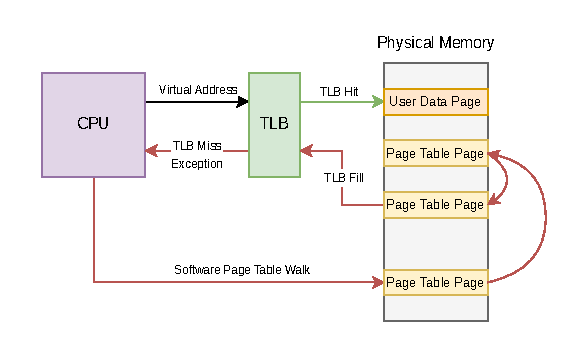
\includegraphics[scale=1.5]{figures/theory_sw_ptw.pdf}
    \caption[Software Page Table Walker]{Instead of transfering control over to the MMU to fill in the missing mapping,
        the TLB Miss exception invokes a software page table walker}
    \label{fig:theory:sw_ptw}
\end{figure*}





\begin{figure*}[t]
    \centering
    \begin{bytefield}[bitwidth=\widefigurewidth/56,bitheight=\widthof{~PBMT~}, bitformatting={\tiny\bfseries}, boxformatting={\centering}]{56}
        \bitheader[endianness=big]{55,30,29,21,20,12,11,0} \\
        \bitbox{26}{PPN[2]} &
        \bitbox{9}{PPN[1]} &
        \bitbox{9}{PPN[0]} &
        \bitbox{12}{Page Offset}\\
    \end{bytefield}
    \caption[RISC-V Sv39 Physical Address]{RISC-V Sv39 Physical Address}
    \label{fig:theory:sv39pa}
\end{figure*}


\begin{figure*}[t]
    \centering
    \begin{bytefield}[bitwidth=\widefigurewidth/64,bitheight=\widthof{~PBMT~}, bitformatting={\tiny\bfseries}, boxformatting={\centering}]{64}
        \bitheader[endianness=big]{63,60,59,44,43,0} \\
        \bitbox{4}{Mode} &
        \bitbox{16}{ASID} &
        \bitbox{44}{PPN} \\
    \end{bytefield}
    \caption[RISC-V Sv39 \texttt{satp} CSR]{RISC-V Sv39 \texttt{satp} CSR}
    \label{fig:theory:sv39satp}
\end{figure*}



% Source Description Stuff - maybe extra chapter, or in way less detail


% -------------------------------------------------------------------------------------------------

\todo{merge this with overview and provide this sort of explanation as a introduction to the implementation part}
\section{Programming Platform}
\subsection{QEMU}
The \texttt{softtlb} design approach requires the CPU to throw an exception when the TLB misses. There is
currently neither a RISC-V platform that supports nor a extension to the RISC-V that specifies that behavior.\\
The logical consequence is to use an emulator and implement the required functionality.\\
This paper uses the QEMU emulator as a foundation for the implementation. QEMU supports a big range of
different platforms and is thus not the simplest source to modify. Additionally, detailed documentation
on internal structures is sparse.\\
However, QEMU does support a lot of features and extensions of the RISC-V target and is quite performant
\cite{bellard2005QEMU}.

% -------------------------------------------------------------------------------------------------

%This section is important for the rationale on choosing a format of the CSRs
%Vielleicht sollte dieser Teil einfach erst im hinblick auf replacement policies Dikutiert werden
% In meinem Programmiermodell ist ja der TLB nichts weiter als ein Indiziertes array von daten, 
% Weitere Aspekte sind ja hier erst mal out of scope
\subsubsection{TLB}
% What type of cache modeled? - direct mapped, associative?

\todo{description of QEMU TLB structure in fundamentals, theory or implementation?}
% Does the QEMU tlb implementation impact the theory? -> It should not
%   It only has impact once we have to decide on a specific format for the tlbh and tlbl csrs
%   But I can put all the theoretical parts into theory, so ASID etc
%   and the modification of the theory based on concrete hardware can come into the impl chapter
%       -> mmuidx and stuff


% -------------------------------------------------------------------------------------------------


\subsection{xv6-riscv}
xv6 is a simple teaching operating system loosely following the design of Unix Version 6 \cite{cox2011xv6}.
It is used to teach an operating systems course and does not contain the complexities of real-life
operating systems.

% -------------------------------------------------------------------------------------------------
%                                    SECTION Source Description
% -------------------------------------------------------------------------------------------------
\section{Source Overview}
The implementation consists of two fundamental parts:
The extension of RISC-V ISA emulated by QEMU and the implementation of a
TLB Miss Handler.

% -------------------------------------------------------------------------------------------------

\subsection{QEMU}
\texttt{cputlb.c} found in \texttt{accel/tcg} contains the TLB-handling logic for all
emulation targets; from there, target-specific functions for TLB management are called.
The target-specific functions are implemented in \texttt{target/riscv}.\\
Every target needs to implement the functions in the \texttt{TCGCPUOps} struct in
\texttt{include/hw/core/tcg-cpu-ops.h}. This struct is part of the glue that connects the target-independent
Tiny Code Generator (TCG) backend with the target-specific functions and structures.

% -------------------------------------------------------------------------------------------------

\todo{sequence diagram for function calls accross the QEMU repository}

% -------------------------------------------------------------------------------------------------

% TCGCPUOps struct
% TODO Ausgangspunkt sollte die mmu_lookup1 funktion sein!
The \texttt{TCGCPUOps} struct includes a function pointer named \texttt{tlb\_fill}. The function is called
when MMU lookups to the TLB and QEMU's victim TLB fail.
For the riscv target, the function \texttt{riscv\_cpu\_tlb\_fill} is assigned to the \texttt{tlb\_fill}
function pointer in \texttt{target/riscv/tcg/tcg-cpu.c}.\\
The implementation for \texttt{riscv\_cpu\_tlb\_fill} is in \texttt{target/riscv/cpu\_helper.c}. This is a common
file to be found in a target-specifc directory and contains general functionality to implement the \texttt{TCGCPUOps} struct.\\


\todo{explain PTE}

% -------------------------------------------------------------------------------------------------

\subsection{xv6}



% -------------------------------------------------------------------------------------------------
%                                END OF SECTION - Source Description
% -------------------------------------------------------------------------------------------------

